\documentclass{article}%
\usepackage[T1]{fontenc}%
\usepackage[utf8]{inputenc}%
\usepackage{lmodern}%
\usepackage{textcomp}%
\usepackage{lastpage}%
\usepackage{authblk}%
\usepackage{graphicx}%
%
\title{Multidrug resistance protein MdtM adds to the repertoire of antiporters involved in alkaline pH homeostasis in Escherichia coli}%
\author{Megan Jordan}%
\affil{Institute of Pharmacology, Toxicology and Pharmacy, Ludwig{-}Maximilians{-}University, Munich, Germany}%
\date{01{-}01{-}2013}%
%
\begin{document}%
\normalsize%
\maketitle%
\section{Abstract}%
\label{sec:Abstract}%
SAN DIEGO {-} Decreasing inflammatory mediators are on the rise in the neuropathy that afflicts Type 2 diabetes, according to a new study from the Juvenile Diabetes Research Foundation.\newline%
While the study's findings are preliminary and have not been completely verified, preliminary work suggested an overall increase in inflammatory mediators {-} called cytokines {-} and their interactions with certain functions that affect the body's response to nerve dysfunction.\newline%
During a severe spike in inflammatory mediators in the blood, diabetic complications can mount {-} including a syndrome called chronic nerve disease (CHRD), which is tied to errors in nerve function in diabetes. CHRD symptoms can be deadly, leading to heart attacks and stroke.\newline%
As the team at the Diabetes Center at Scripps Research Institute examined tissue samples from healthy volunteers, they found that several inflammatory mediators (known as interleukin{-}6, interleukin{-}8, interleukin{-}15, interleukin{-}26 and interleukin{-}24) were produced in greater levels in areas where the body's responses to nerve injury was disrupted.\newline%
Among the inflammatory mediators produced in this "resource{-}dense" area are interleukin{-}9, interleukin{-}13, interleukin{-}24, interleukin{-}26, interleukin{-}27, interleukin{-}32, interleukin{-}35, interleukin{-}32, interleukin{-}37, interleukin{-}34, interleukin{-}34, interleukin{-}36, interleukin{-}33, interleukin{-}33, interleukin{-}34, interleukin{-}35, interleukin{-}34, interleukin{-}36, interleukin{-}35, interleukin{-}38, interleukin{-}39, interleukin{-}38, interleukin{-}39, interleukin{-}37, interleukin{-}36, interleukin{-}36, interleukin{-}36, interleukin{-}36, interleukin{-}36, interleukin{-}36, interleukin{-}36, interleukin{-}36, interleukin{-}36, interleukin{-}36, interleukin{-}36, interleukin{-}36, interleukin{-}36, interleukin{-}36, interleukin{-}36, interleukin{-}36, interleukin{-}36, interleukin{-}36, interleukin{-}36, interleukin{-}36, interleukin{-}36, interleukin{-}36, interleukin{-}36, interleukin{-}36, interleukin{-}36, interleukin{-}36, interleukin{-}36, interleukin{-}36, interleukin{-}36, interleukin{-}36, interleukin{-}36, interleukin{-}36, interleukin{-}36, interleukin{-}36, interleukin{-}36, interleukin{-}36, interleukin{-}36, interleukin{-}36, interleukin{-}36, interleukin{-}36, interleukin{-}36, interleukin{-}36, interleukin{-}36, interleukin{-}36, interleukin{-}36, interleukin{-}36, interleukin{-}36, interleukin{-}36, interleukin{-}36, interleukin{-}36, interleukin{-}36, interleukin{-}36, interleukin{-}36, interleukin{-}36, interleukin{-}36, interleukin{-}36, interleukin{-}36, interleukin{-}36, interleukin{-}36, interleukin{-}36, interleukin{-}36, interleukin{-}36, interleukin{-}36, interleukin{-}36, interleukin{-}36, interleukin{-}36, interleukin{-}36, interleukin{-}36, interleukin{-}36, interleukin

%
\subsection{Image Analysis}%
\label{subsec:ImageAnalysis}%


\begin{figure}[h!]%
\centering%
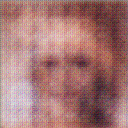
\includegraphics[width=150px]{500_fake_images/samples_5_449.png}%
\caption{A Man Is Holding A Cat In His Arms}%
\end{figure}

%
\end{document}